\section*{Appendix A}
\lstset{
 upquote=true,
 showspaces=false,
 showtabs=false,
 frame=none,
 tabsize=2,
 breaklines=true,
 numbers=none,
 showstringspaces=false,
 breakatwhitespace=true,
 escapeinside={(*@}{@*)},
 keywordstyle=\bfseries,
 basicstyle=\scriptsize\ttfamily,
 moredelim=**[is][\color{red}]{@}{@},
}

In this appendix are reported the answers to the questions proposed in all the
activities included in this paper.


\subsection*{Activity 1}

\subsubsection*{Task 7 - Step 2}
\textit{Test the created topology: verify the network connectivity between all hosts.
Write in the lines below the commands you used and the results you obtained.}
\begin{figure}[htb]
	\centering
	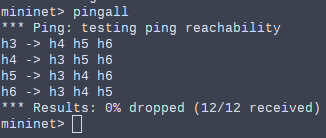
\includegraphics[width=0.5\linewidth]{img/task-7-step-2.png}
\end{figure}



\subsubsection*{Task 7 - Step 3}
\textit{Verify that the bandwidth and the delay of each link comply with the values
specified in the topology diagram shown in figure 1. Write in the lines below
the commands you used and the results you obtained.}

\begin{itemize}
  \item \code{h3 ping h4 -c 10}

  Output:
  \begin{lstlisting}
  --- 10.0.0.2 ping statistics ---
  5 packets transmitted, 5 received, 0% packet loss, time 4006ms
  rtt min/avg/max/mdev = 23.186/25.264/26.760/1.507 ms
  \end{lstlisting}
  The average RTT is approximately 20ms, wich comply the link delays values
  specified in the topology diagram. The same proceeding can be used to test the
  delay of all the others links.

  It's important to point out that the link delay between the two switches doesn't
  comply with the topology diagram: this behavior is however acceptable and it's due to
  the fact that in Mininet the switches are by default run in the same network
  namespace inside the kernel space, therefore they communicate to each other
  without using the created link which has the performance parameters specified
  in the Python script.

  \item \code{iperf h3 h4}

  Output:
  \begin{lstlisting}
  *** Iperf: testing TCP bandwidth between h3 and h6
  *** Results: ['4.75 Mbits/sec', '6.23 Mbits/sec']
  \end{lstlisting}

  The same proceeding can be used to test the bandwidth between all nodes.
\end{itemize}



\subsubsection*{Task 8 - Question 1}
\textit{What are the advantages of having more controllers instead of
one single controller which serves all the switches of the network?}




\subsubsection*{Task 8 - Question 2}
\textit{Would the fault tolerance of the netowrk shown in figure 1
change if we used only one controller (linked to both the switches)
instead of two?}




\subsubsection*{Task 8 - Question 3}
\textit{In this activity the topology shown in figure 1 was implemented
assuming that the two controllers were local controllers. How
would you have to change the Python script you created in this
activity in order to use remote controllers instead of local ones?
(Hint: see reference [5])}

The changes that has to be applied to the Python script are marked with the red
colour in the listing below.

\lstset{
 upquote=true,
 showspaces=false,
 showtabs=false,
 frame=single,
 tabsize=2,
 breaklines=true,
 numbers=left,
 showstringspaces=false,
 breakatwhitespace=true,
 escapeinside={(*@}{@*)},
 keywordstyle=\bfseries,
 basicstyle=\scriptsize\ttfamily,
 moredelim=**[is][\color{red}]{@}{@},
}
\begin{minipage}{\linewidth}
\begin{lstlisting}
#!/usr/bin/Python
from mininet.net import Mininet
from mininet.node import Controller, OVSSwitch, @RemoteController@
from mininet.cli import CLI
from mininet.log import setLogLevel, info
from mininet.link import TCLink

def multiControllerNet():
    net = Mininet( controller=Controller, switch=OVSSwitch, link=TCLink )

    info( "*** Creating hosts\n" )
    h1 = net.addHost('h3')
    h2 = net.addHost('h4')
    h3 = net.addHost('h5')
    h4 = net.addHost('h6')

    info( "*** Creating switches\n" )
    s1 = net.addSwitch( 's1' )
    s2 = net.addSwitch( 's2' )

    info( "*** Creating links\n" )
    net.addLink( h1, s1, bw=5, delay='5ms' )
    net.addLink( h2, s1, bw=5, delay='5ms' )
    net.addLink( h3, s2, bw=5, delay='5ms' )
    net.addLink( h4, s2, bw=5, delay='5ms' )
    net.addLink( s1, s2, bw=10, delay='2ms' )

    info( "*** Creating (reference) controllers\n" )
    c0 = net.addController( 'c0', @controller=RemoteController, ip='127.0.0.1'@, port=6633 )
    c1 = net.addController( 'c1', @controller=RemoteController, ip='127.0.0.1'@, port=6634 )

    info( "*** Starting network\n" )
    net.build()
    c0.start()
    c1.start()
    s1.start( [ c0 ] )
    s2.start( [ c1 ] )

    info( "*** Running CLI\n" )
    CLI( net )

    info( "*** Stopping network\n" )
    net.stop()

if __name__ == '__main__':
    setLogLevel( 'info' )
    multiControllerNet()
\end{lstlisting}
\end{minipage}

For simplicity it has been assumed that the two remote controllers are running on the same machine on
which Mininet is running, therefore the ip \code{127.0.0.1} has been used (if the
controllers had been on different machines the relative IP should have been used).




\subsubsection*{Task 8 - Question 4}
\textit{How could we improve the fault tolerance of the netowork shown
in figure 1 making minor changes to the Python script used?}







\lstset{
 upquote=true,
 showspaces=false,
 showtabs=false,
 frame=none,
 tabsize=2,
 breaklines=true,
 numbers=none,
 showstringspaces=false,
 breakatwhitespace=true,
 escapeinside={(*@}{@*)},
 keywordstyle=\bfseries,
 basicstyle=\scriptsize\ttfamily,
 moredelim=**[is][\color{red}]{@}{@},
}
\subsection*{Activity 2}
\subsubsection*{Task 5 - Step 2}
\textit{Test the created topology: verify the network connectivity between all hosts.
Write in the lines below the commands you used and the results you obtained.}
\begin{figure}[htb]
	\centering
	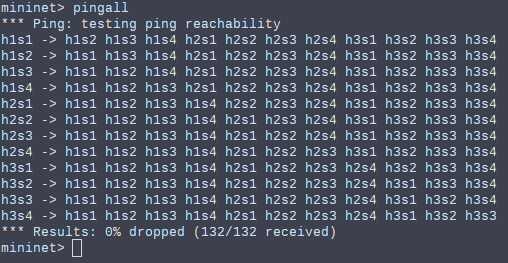
\includegraphics[width=0.8\linewidth]{img/activity-2-task-5-step-2.png}
\end{figure}


\subsubsection*{Task 5 - Step 3}
\textit{Verify the bandwidth and the delay between the hosts h1s1 and h3s4. Write
in the lines below the commands you used and the results you obtained.}
\begin{itemize}
  \item \code{iperf h1s1 h3s4}

  Result:
  \begin{lstlisting}
  *** Iperf: testing TCP bandwidth between h1s1 and h3s4
  *** Results: ['4.25 Gbits/sec', '4.26 Gbits/sec']
  \end{lstlisting}

  \item \code{h1s1 ping h3s4 -c 10}

  Result:
  \begin{lstlisting}
  --- 10.0.0.12 ping statistics ---
  10 packets transmitted, 10 received, 0% packet loss, time 9006ms
  rtt min/avg/max/mdev = 0.107/4.042/24.062/7.490 ms
  \end{lstlisting}
\end{itemize}
